Pro potřeby této práce byly vytvořeny 2 aplikace a 2 knihovny. První aplikace je
demonstrační aplikací k~měřicímu vozu, tato aplikace pouze zobrazuje naměřená
data. Druhá aplikace je o~mnoho komplexnější a řeší přímo problém automatické
kalibrace.

\section{Volba nástrojů}
\label{sec:sw-nastroje}

Zásadní otázkou, kterou je třeba zodpovědět před vytváření programu, je
jaký programovací jazyk a případně framework zvolit. Zde měl autor poměrně
jasný požadavek na programovací jazyk: jazyk musí mít poměrně silný typový
systém tak, aby netriviální množství kontrol proběhlo již během překladu.
Důvodem pro tento argument je fakt, že autor vyrábí aplikaci, které je tzv.
\textit{kritická}. V~kontextu této práce to znamená, že vlivem chyby
v~aplikaci může dojít k~materiálním škodám na kalibrovaném modelu (ceny
vybraných malosériových modelů se pohybují až v~desítkách tisíc Kč).

Dalším přirozeným požadavkem bylo, aby programovací jazyk měl rozumnou podporu
pro komunikaci se sériovým portem, neboť toto rozhraní bude použito jak pro
komunikaci s~měřicím vozem, tak pro komunikaci s~digitální centrálou DCC.

Dalším kritériem při výběru programovacího jazyka byla jeho předchozí znalost
autorem práce. Zejména u~kritických aplikací je totiž nanejvýš důležité, aby
programátor přesně věděl, co dělá.

Při rozmýšlení nad technologií aplikace bylo rozhodnuto, že program by měl
mít grafické uživatelské rozhraní (GUI), neboť je nanejvýš vhodné zobrazovat
přehledně aktuální průběh kalibrace a neboť jsou běžní uživatelé na GUI
aplikace zvyklí.

Zásadní je pak otázka typu aplikace. Autor uvažoval aplikace desktopové,
mobilní, webové a dokonce i~embedded! Embedded aplikace s~sebou nesou tu
nevýhodu, že obsluha s~aplikací typicky nemůže příliš interagovat, u~mobilních
aplikací je v~kontextu této práce omezující zejména zobrazovací plocha
zařízení, na kterou se jednoduše nevejde tolik dat, kolik by aplikace chtěla
zobrazovat. Navíc vývoj pro jiné zařízení, než na kterém se kód píše, vždy
přináší nějakou režii navíc.

Výhodou webové aplikace by byla snadná přenositelnost na jiné počítače,
aplikace by dokonce mohla být přístupná i~z~mobilního zařízení. Bohužel, proti
tomuto formátu aplikace hovoří fakt, že autor práce nemá s~webovými aplikacemi
dostatečné zkušenosti a už vůbec si netroufá v~nich psát kritický kód.
Oproti desktopovým aplikacím jsou interaktivní webové aplikace navíc o~něco
složitější (zejména co se týče předávání signálů z~GUI).

Další možností pak byly desktopové aplikace. Vzhledem k~požadavkům uvedeným
výše a k~faktu, že se jedná už o~poněkud rozsáhlejší projekt, jako nejvhodnější
se autorovi jevil jazyk \texttt{C++} s~použitím frameworku \texttt{Qt}.
Argumentem pro tento framework byly dobré osobní reference, které na
\texttt{Qt} autor práce dostal od kolegů. Ukázalo se také, že \texttt{Qt} poskytují
nejen výbornou multiplatformní podporu pro GUI, ale také stejně dobrou
multiplatformní podporu pro sériový port. Bylo tedy rozhodnuto, že výsledná
aplikace bude psána v~programovacím jazyce \texttt{C++} (konkrétně
\texttt{C++14}) za použití frameworku \texttt{Qt} a bude multiplatformní
(minimálně mezi OS \texttt{Windows} a \texttt{Linux}).

\section{WSM Speed Reader}
\label{sec:sw-wsm-speed-reader}

První aplikací je \textit{WSM Speed Reader} -- jednoduchý zobrazovač vyčtených
dat. Aplikace se skládá z~jednoho okna a je především typu
\textit{proof of concept}. GUI aplikace je zachyceno na obrázku
\ref{fig:wsm-speed-reader-gui}.

\begin{figure}[h]
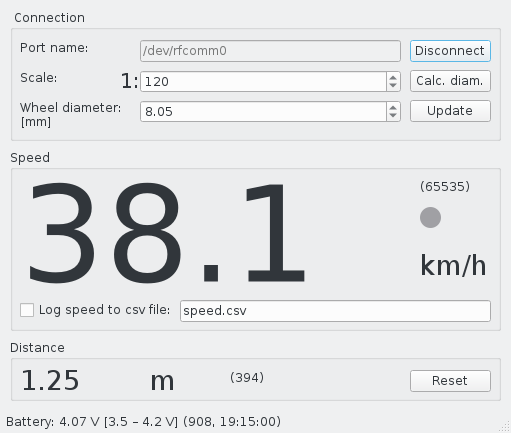
\includegraphics[width=0.7\textwidth]{data/speed_reader_screenshot.png}
\caption{GUI programu WSM Speed Reader.}
\label{fig:wsm-speed-reader-gui}
\end{figure}

Aplikace se připojuje k~sériovému portu, ze zadaných parametrů vypočítává
rychlost a ujetou vzdálenost vozidla a tyto údaje zobrazuje. Umožňuje ukládání
vyčtených dat do souboru (především pro vývoj) a ukládání nastavení aplikace
do konfiguračního souboru. Aplikace je volně dostupná pod licencí Apache
License v2.0 \cite{wsm-speed-reader}.

Při programování této aplikace bylo rozhodnuto vyčlenit knihovnu umožňující
komunikaci s~měřicím vozem WSM do samostatného repozitáře. Knihovna se skládá
hlavičkového souboru \texttt{wsm.h}, který definuje API třídy \texttt{Wsm},
implementace této knihovny (v~samostatném \texttt{cpp} souboru) a pomocných
souborů. Knihovna je k dispozici
online\footnote{\url{https://github.com/kmzbrnoI/wsm-lib-cpp-qt}}, bylo k ní
vytvořeno srozumitelné README a dodány všechny náležitosti samostatné stojícího
projektu.

I přes původní snahy je nutné pro užití knihovny v projektu využít frameworku
\texttt{Qt} a to zejména kvůli implementaci sériového portu.

\section{Automatic Calibration}
\label{sec:sw-wsm-auto-calib}
